\section{PREDNOSTI I OGRANIČENJA}
Uvođenje autonomnih viličara u skladišne i proizvodne sustave donosi značajne promjene u načinu na koji se planiraju i izvršavaju intralogistički procesi. Kako bi se donijela opravdana odluka o implementaciji, potrebno je sveobuhvatno sagledati operativne prednosti, ali i ekonomske te tehničko-tehnološke aspekte i ograničenja koja prate rad ovih sustava.

\subsection{Prednosti}
Primarni pokretač automatizacije u intralogistici je postizanje visoke razine operativne učinkovitosti i eliminacija slabosti karakterističnih za ljudski rad. Ključne prednosti uključuju:
\begin{enumerate}
    \item \textbf{Povećanje produktivnosti i neprekidan rad (24/7):} Autonomni viličari mogu raditi neprekidno bez potrebe za stankama za odmor, hranu, bolovanja ili promjene smjena. Vrijeme zastoja svedeno je isključivo na planirano održavanje i automatsko punjenje baterija (engl. \textit{opportunity charging}), koje se obično provodi u kratkim intervalima kada vozilo nema aktivnih zadataka. To omogućuje konstantan protok materijala i maksimalno iskorištenje skladišnih kapaciteta, posebno u noćnim smjenama.
    \item \textbf{Povećana sigurnost i smanjenje broja nesreća:} Ljudski faktor je glavni uzrok nesreća u skladištima (brza vožnja, umor, nepažnja pri ubadanju paleta). Budući da se autonomni viličari kreću po precizno definiranim putanjama i opremljeni su sigurnosnim skenerima razine PLd, oni se trenutačno zaustavljaju u prisutnosti pješaka ili prepreka. Time se rizik od ozljeda radnika i oštećenja skupih skladišnih regala svodi na minimum.
    \item \textbf{Ublažavanje nedostatka radne snage:} Logistički sektor se diljem svijeta suočava s kroničnim nedostatkom kvalificiranih operatera viličara, uz istovremeno visoku fluktuaciju radne snage. Automatizacija omogućuje poduzećima da stabiliziraju svoje procese i preusmjere postojeće radnike na složenije zadatke poput kontrole kvalitete, prepakiranja ili upravljanja samim sustavom.
    \item \textbf{Preciznost i sljedivost (Traceability):} Svaki nalog za prijenom palete prati se digitalno u realnom vremenu. Integracija viličara s WMS sustavom eliminira mogućnost ljudske pogreške pri odlaganju robe na pogrešnu lokaciju, čime se postiže stopostotna točnost inventara.
\end{enumerate}

\subsection{Ekonomska usporedba i povrat investicije (ROI)}
Donošenje odluke o implementaciji autonomnih viličara zahtijeva detaljnu financijsku procjenu. Dok klasični viličari predstavljaju manju početnu investiciju uz visoke i kontinuirane operativne troškove, autonomni sustavi zahtijevaju značajan početni kapital (CAPEX) koji se amortizira kroz dramatično smanjenje operativnih troškova (OPEX) tijekom životnog vijeka sustava.

Za potrebe ove usporedbe definirane su metodološke pretpostavke i financijski iznosi prikupljeni iz službenih cjenika i tehničko-komercijalnih specifikacija vodećih proizvođača Toyota Material Handling (serija Autopilot i sustav T-ONE) \cite{toyota} i Jungheinrich AG (Logistics Interface sustavi) \cite{jungheinrich}, te podataka Državnog zavoda za statistiku (DZS) \cite{dzs} i Eurostata \cite{eurostat} o cijenama rada u logističkom sektoru za 2024. i 2025. godinu.
Financijska procjena temelji se na sljedećim pretpostavkama:
\begin{itemize}
    \item \textbf{Životni vijek projekta ($N$):} Analiza se provodi za razdoblje od $N = 5$ godina, što odgovara uobičajenom ciklusu tehnološke amortizacije intralogističke opreme.
    \item \textbf{Opseg sustava:} Uspoređuje se rad jednog klasičnog visokopodiznog viličara (reach truck) i jednog ekvivalentnog autonomnog viličara (AMR).
    \item \textbf{Operativni režim:} Pretpostavlja se kontinuirani rad u 3 smjene (ukupno 24 sata dnevno), 250 radnih dana godišnje. To iznosi ukupno 6.000 radnih sati godišnje po vozilu.
    \item \textbf{Trošak rada:} Prema podacima DZS-a i Eurostata \cite{dzs, eurostat}, prosječni ukupni trošak rada (Bruto II) skladišnog operatera viličara u Republici Hrvatskoj iznosi 20.000 EUR godišnje. Rad u 3 smjene zahtijeva 3 operatera (3 FTE), što iznosi ukupno 60.000 EUR godišnje po klasičnom viličaru.
    \item \textbf{Diskontna stopa ($r$):} Koristi se standardna industrijska diskontna stopa od $r = 8\%$ ($0,08$) za proračun vremenske vrijednosti novca sukladno preporukama u literaturi o upravljanju logističkim troškovima \cite{bowersox}.
\end{itemize}

Struktura troškova (CAPEX i OPEX) prikazana je u tablici \ref{tab:tco_detaljno}:
\begin{enumerate}
    \item \textbf{CAPEX (Kapitalni troškovi):} Nabavna cijena klasičnog viličara iznosi 35.000 EUR \cite{toyota, jungheinrich}. Nabavni trošak autonomnog viličara iznosi 95.000 EUR s uključenom senzorikom, čemu se pribrajaju troškovi softverskih licenci i integracije s WMS sustavom (25.000 EUR) te usluga mapiranja skladišta i postavljanja sigurnosnih zona (5.000 EUR), što daje ukupni početni CAPEX od 125.000 EUR \cite{toyota, jungheinrich}.
    \item \textbf{OPEX (Operativni troškovi):} Godišnji trošak održavanja i servisa iznosi 4.000 EUR za klasični viličar, dok je za autonomni viličar procijenjen na 8.000 EUR zbog ugovora o održavanju napredne senzorike i softvera \cite{toyota, jungheinrich}. Trošak električne energije iznosi 1.500 EUR za klasični, odnosno 1.800 EUR za autonomni viličar (dodatna potrošnja ugrađenih industrijskih računala). Trošak šteta na robi i regali iznosi 5.000 EUR godišnje za klasični viličar pod utjecajem ljudskih pogrešaka, dok se kod autonomnog vozila smanjuje na 500 EUR godišnje \cite{bowersox}.
\end{enumerate}

U tablici \ref{tab:tco_detaljno} prikazana je detaljna struktura i usporedba troškova.

\begin{table}[h]
\centering
\caption{Detaljna usporedba troškova (CAPEX i OPEX) za životni vijek od 5 godina}
\label{tab:tco_detaljno}
\begin{tabularx}{\textwidth}{|l|r|r|}
\hline
\textbf{Stavka troška} & \textbf{Klasični viličar (3 smjene)} & \textbf{Autonomni viličar (AMR)} \\ \hline
\textbf{Nabavna cijena vozila} & 35.000 EUR & 95.000 EUR \\ \hline
\textbf{Softverske licence i integracija} & 0 EUR & 25.000 EUR \\ \hline
\textbf{Mapiranje i sigurnosne zone} & 0 EUR & 5.000 EUR \\ \hline
\textbf{Ukupni CAPEX (početna investicija)} & \textbf{35.000 EUR} & \textbf{125.000 EUR} \\ \hline
\textbf{Godišnji trošak rada (3 FTE)} & 60.000 EUR / god & 0 EUR / god \\ \hline
\textbf{Godišnji trošak održavanja} & 4.000 EUR / god & 8.000 EUR / god \\ \hline
\textbf{Godišnji trošak električne energije} & 1.500 EUR / god & 1.800 EUR / god \\ \hline
\textbf{Godišnji trošak šteta (roba/regali)} & 5.000 EUR / god & 500 EUR / god \\ \hline
\textbf{Ukupni godišnji OPEX} & \textbf{70.500 EUR / god} & \textbf{10.300 EUR / god} \\ \hline
\end{tabularx}
\end{table}

Za ocjenu ekonomske opravdanosti projekta implementacije autonomnog viličara u odnosu na klasični, koriste se tri temeljna financijska indikatora: TCO, NPV i ROI.

\subsubsection{Ukupni troškovi vlasništva (TCO)}
TCO predstavlja zbroj početne investicije i diskontiranih operativnih troškova tijekom životnog vijeka projekta:
\begin{equation}
    TCO = CAPEX + \sum_{t=1}^{N} \frac{OPEX_t}{(1 + r)^t}
\end{equation}
Za faktor diskontiranja pri $N=5$ i $r=0,08$ vrijedi:
\begin{equation*}
    \sum_{t=1}^{5} \frac{1}{(1,08)^t} = 0,9259 + 0,8573 + 0,7938 + 0,7350 + 0,6806 = 3,9927
\end{equation*}
Uvrštavanjem vrijednosti iz tablice \ref{tab:tco_detaljno} dobivamo:
\begin{align}
    TCO_{\text{man}} &= 35.000 + 70.500 \cdot 3,9927 = 35.000 + 281.485 = 316.485\text{ EUR} \\
    TCO_{\text{aut}} &= 125.000 + 10.300 \cdot 3,9927 = 125.000 + 41.125 = 166.125\text{ EUR}
\end{align}
Usporedba pokazuje da je ukupni trošak vlasništva autonomnog viličara tijekom 5 godina manji za \textbf{150.360 EUR} u odnosu na klasični viličar, unatoč znatno većoj početnoj investiciji.

\subsubsection{Neto sadašnja vrijednost (NPV)}
NPV proračunava neto financijski efekt investicije u autonomno vozilo u odnosu na klasično, svodeći sve buduće neto uštede na sadašnju vrijednost:
\begin{equation}
    NPV = -CF_0 + \sum_{t=1}^{N} \frac{CF_t}{(1 + r)^t}
\end{equation}
gdje su:
\begin{itemize}
    \item $CF_0$ — Diferencijalna početna investicija:
    \begin{equation*}
        CF_0 = CAPEX_{\text{aut}} - CAPEX_{\text{man}} = 125.000 - 35.000 = 90.000\text{ EUR}
    \end{equation*}
    \item $CF_t$ — Godišnja neto ušteda ostvarena smanjenjem operativnih troškova:
    \begin{equation*}
        CF_t = OPEX_{\text{man}} - OPEX_{\text{aut}} = 70.500 - 10.300 = 60.200\text{ EUR}
    \end{equation*}
\end{itemize}
Uvrštavanjem u formulu dobivamo:
\begin{equation}
    NPV = -90.000 + 60.200 \cdot 3,9927 = -90.000 + 240.360 = 150.360\text{ EUR}
\end{equation}
Budući da je NPV izrazito pozitivan ($NPV > 0$), projekt je s financijskog aspekta potpuno opravdan i stvara dodatnu vrijednost za poduzeće.

\subsubsection{Povrat investicije (ROI) i razdoblje povrata (PBP)}
ROI izražava profitabilnost projekta kao omjer ukupnih diskontiranih ušteda i početne investicije:
\begin{equation}
    ROI = \frac{TCO_{\text{man}} - TCO_{\text{aut}}}{CAPEX_{\text{aut}}} \cdot 100\% = \frac{316.485 - 166.125}{125.000} \cdot 100\% = 120,29\%
\end{equation}
Jednostavno razdoblje povrata (engl. \textit{Payback Period}) predstavlja vrijeme potrebno da se kroz godišnje operativne uštede povrati diferencijalna investicija:
\begin{equation}
    PBP = \frac{CF_0}{CF_t} = \frac{90.000}{60.200} = 1,495\text{ godina} \approx 18\text{ mjeseci}
\end{equation}
Investicija se u potpunosti isplati za manje od godinu i pol dana rada u trosmjenskom sustavu.

\subsubsection{Analiza osjetljivosti (Sensitivity Analysis)}
Kako bi se procijenio rizik investicije u uvjetima promjene tržišnih parametara, provedena je analiza osjetljivosti za dva alternativna scenarija:
\begin{enumerate}
    \item \textbf{Scenarij A: Rad u 2 smjene (smanjeni intenzitet rada):}
    Broj radnika se smanjuje na 2 (2 FTE), što smanjuje godišnji trošak rada klasičnog viličara na 40.000 EUR. Ukupni godišnji OPEX klasičnog viličara pada na 50.500 EUR. Godišnja neto ušteda iznosi $CF_t = 50.500 - 10.300 = 40.200$ EUR.
    \begin{align*}
        NPV_A &= -90.000 + 40.200 \cdot 3,9927 = 70.506\text{ EUR} \\
        PBP_A &= \frac{90.000}{40.200} = 2,24\text{ godine} \approx 27\text{ mjeseci}
    \end{align*}
    Investicija ostaje isplativa, no razdoblje povrata se produljuje na nešto više od dvije godine.
    \item \textbf{Scenarij B: Povećanje cijene rada za 15\% (utjecaj inflacije):}
    Trošak rada po radniku raste na 23.000 EUR bruto II godišnje. Trošak rada za 3 smjene iznosi 69.000 EUR. Ukupni godišnji OPEX klasičnog viličara raste na 79.500 EUR. Godišnja neto ušteda iznosi $CF_t = 79.500 - 10.300 = 69.200$ EUR.
    \begin{align*}
        NPV_B &= -90.000 + 69.200 \cdot 3,9927 = 186.295\text{ EUR} \\
        PBP_B &= \frac{90.000}{69.200} = 1,30\text{ godina} \approx 15.5\text{ mjeseci}
    \end{align*}
    Rast cijene rada dodatno ubrzava povrat investicije i povećava ukupnu profitabilnost projekta.
\end{enumerate}

U tablici \ref{tab:senzitivnost} prikazan je usporedni pregled scenarija.

\begin{table}[h]
\centering
\caption{Rezultati analize osjetljivosti projekta automatizacije}
\label{tab:senzitivnost}
\begin{tabularx}{\textwidth}{|l|X|X|X|}
\hline
\textbf{Financijski indikator} & \textbf{Osnovni scenarij (3 smjene)} & \textbf{Scenarij A (2 smjene)} & \textbf{Scenarij B (Rast plaća 15\%)} \\ \hline
\textbf{Godišnja ušteda ($CF_t$)} & 60.200 EUR & 40.200 EUR & 69.200 EUR \\ \hline
\textbf{Neto sadašnja vrijednost (NPV)} & 150.360 EUR & 70.506 EUR & 186.295 EUR \\ \hline
\textbf{Razdoblje povrata (PBP)} & 1,49 godina & 2,24 godine & 1,30 godina \\ \hline
\textbf{Profitabilnost (ROI)} & 120,29\% & 56,40\% & 149,03\% \\ \hline
\end{tabularx}
\end{table}

\begin{figure}[h]
\centering
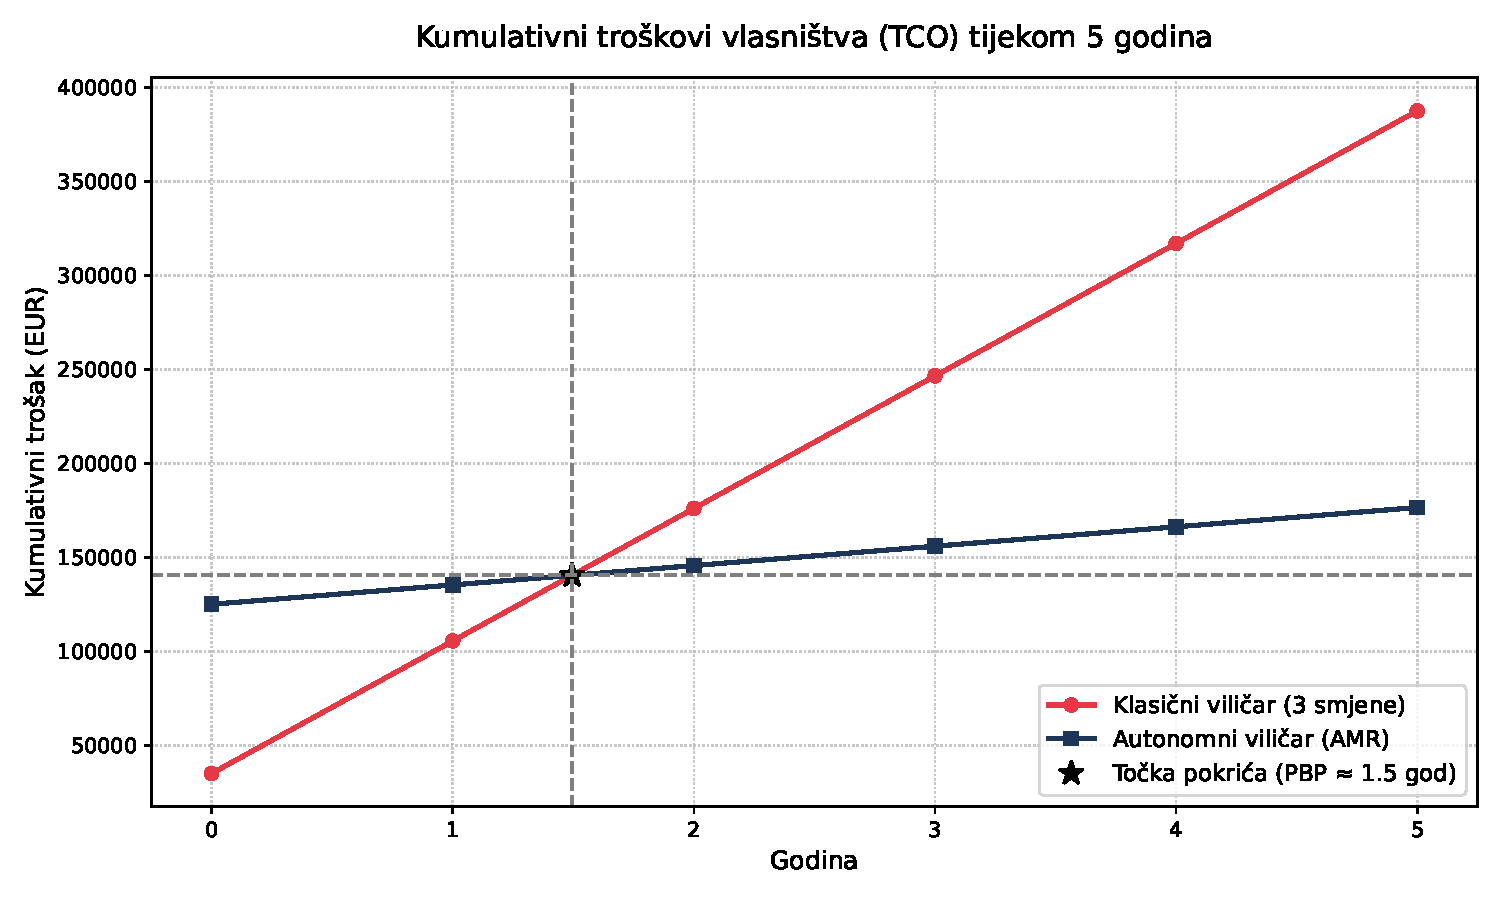
\includegraphics[width=0.9\textwidth]{slike/roi_chart.pdf}
\caption{Kumulativni troškovi vlasništva (TCO) tijekom 5 godina.}
\label{fig:roi_chart}
\end{figure}

Ekonomska analiza jasno pokazuje da je uvođenje autonomnih viličara izrazito opravdano u radnim okruženjima s visokim intenzitetom rada (2 ili više smjena) i visokim udjelom troškova ljudskog rada.

\subsection{Tehničko-tehnološka ograničenja i operativni izazovi}
Unatoč napretku tehnologije, autonomni viličari nisu univerzalno rješenje za sve probleme i zahtijevaju specifične radne uvjete:
\begin{enumerate}
    \item \textbf{Problem Wi-Fi/5G roaminga:} Stalna komunikacija s fleet managerom (npr. T-ONE) preduvjet je za rad. Prilikom kretanja kroz hodnike, viličar mora brzo i bez gubitka paketa prelaziti s jedne Wi-Fi pristupne točke (AP) na drugu. Ako prebacivanje traje dulje od 200 ms, sustav iz sigurnosnih razloga inicira zaustavljanje vozila. Rješavanje ovog problema zahtijeva značajne investicije u robusnu industrijsku mrežnu infrastrukturu.
    \item \textbf{Kvaliteta skladišnih podova (DIN 18202):} Prirodna navigacija i fuzija senzora uvelike se oslanjaju na odometriju. Ako su podovi neravni, imaju pukotine ili nagibe koji odstupaju od standarda DIN 18202, kotači viličara proklizavaju. To dovodi do akumulacije pogreške u Kalmanovom filtru i gubitka lokalizacije, kao i do opasnih vibracija tereta na velikim visinama.
    \item \textbf{Utjecaj okolišnih uvjeta:} Optoelektronički senzori (LiDAR-i i kamere) osjetljivi su na prašinu, vlagu i ekstremne promjene osvjetljenja. U skladištima s visokom koncentracijom suspendiranih čestica (papirna, drvna ili cementna industrija), senzori se moraju učestalo čistiti kako ne bi došlo do lažnih detekcija prepreka i zastoja u radu.
    \item \textbf{Nedostatak kognitivne fleksibilnosti:} Autonomni sustavi slijede stroge algoritamske obrasce. Ako viličar naiđe na stršeći komad plastične folije s palete, on će to prepoznati kao čvrstu prepreku i zaustaviti se, dok bi ljudski vozač procijenio da je prolazak siguran i nastavio vožnju.
\end{enumerate}
